\chapter{Introduction}
\label{sec:intro}

\cleanchapterquote{We are all learning, modifying, or destroying ideas all the time.}{Charles T. Munger}{(American investor.)}


\noindent The university was formed in 1963 as a federation of three existing colleges. The first of these, New Asia College, was established in 1949 by anti-Communist Confucian scholars from Mainland China amid the revolution there. Among the founders were Ch'ien Mu, Tang Junyi, and Tchang Pi-kai. Curriculum focused particularly on Chinese heritage and social concerns. The early years of this school were tumultuous, with the campus relocating several times between rented premises around Kowloon. Academics there were often self-exiled from the mainland and they struggled financially, with students sometimes sleeping on rooftops and teachers foregoing pay to sustain the college. Funds were gradually raised and the school moved to a new campus in Kau Pui Lung, built with the support of the Ford Foundation, in 1956.

\section{Origins}
\subsection{Origins--1}
\noindent The university was formed in 1963 as a federation of three existing colleges. The first of these, New Asia College, was established in 1949 by anti-Communist Confucian scholars from Mainland China amid the revolution there. Among the founders were Ch'ien Mu, Tang Junyi, and Tchang Pi-kai. Curriculum focused particularly on Chinese heritage and social concerns. The early years of this school were tumultuous, with the campus relocating several times between rented premises around Kowloon. Academics there were often self-exiled from the mainland and they struggled financially, with students sometimes sleeping on rooftops and teachers foregoing pay to sustain the college. Funds were gradually raised and the school moved to a new campus in Kau Pui Lung, built with the support of the Ford Foundation, in 1956.

\begin{figure}[t]
\centering
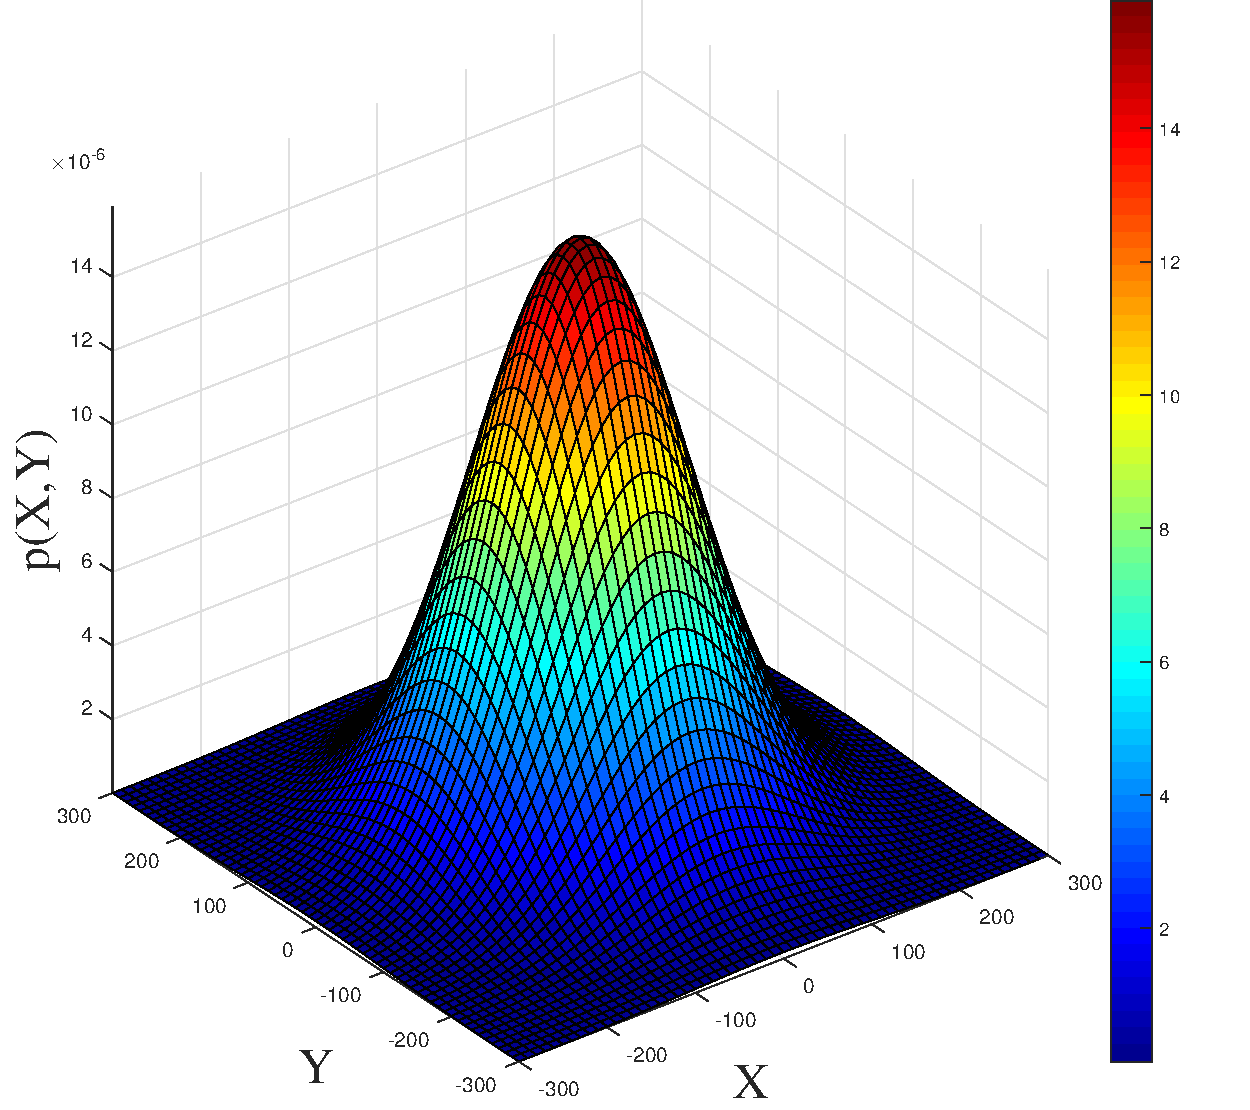
\includegraphics[width=4.5in]{imgs/1}
\caption{imgs/1}
\label{imgs/1}
\end{figure}

\begin{figure}[t]
\centering
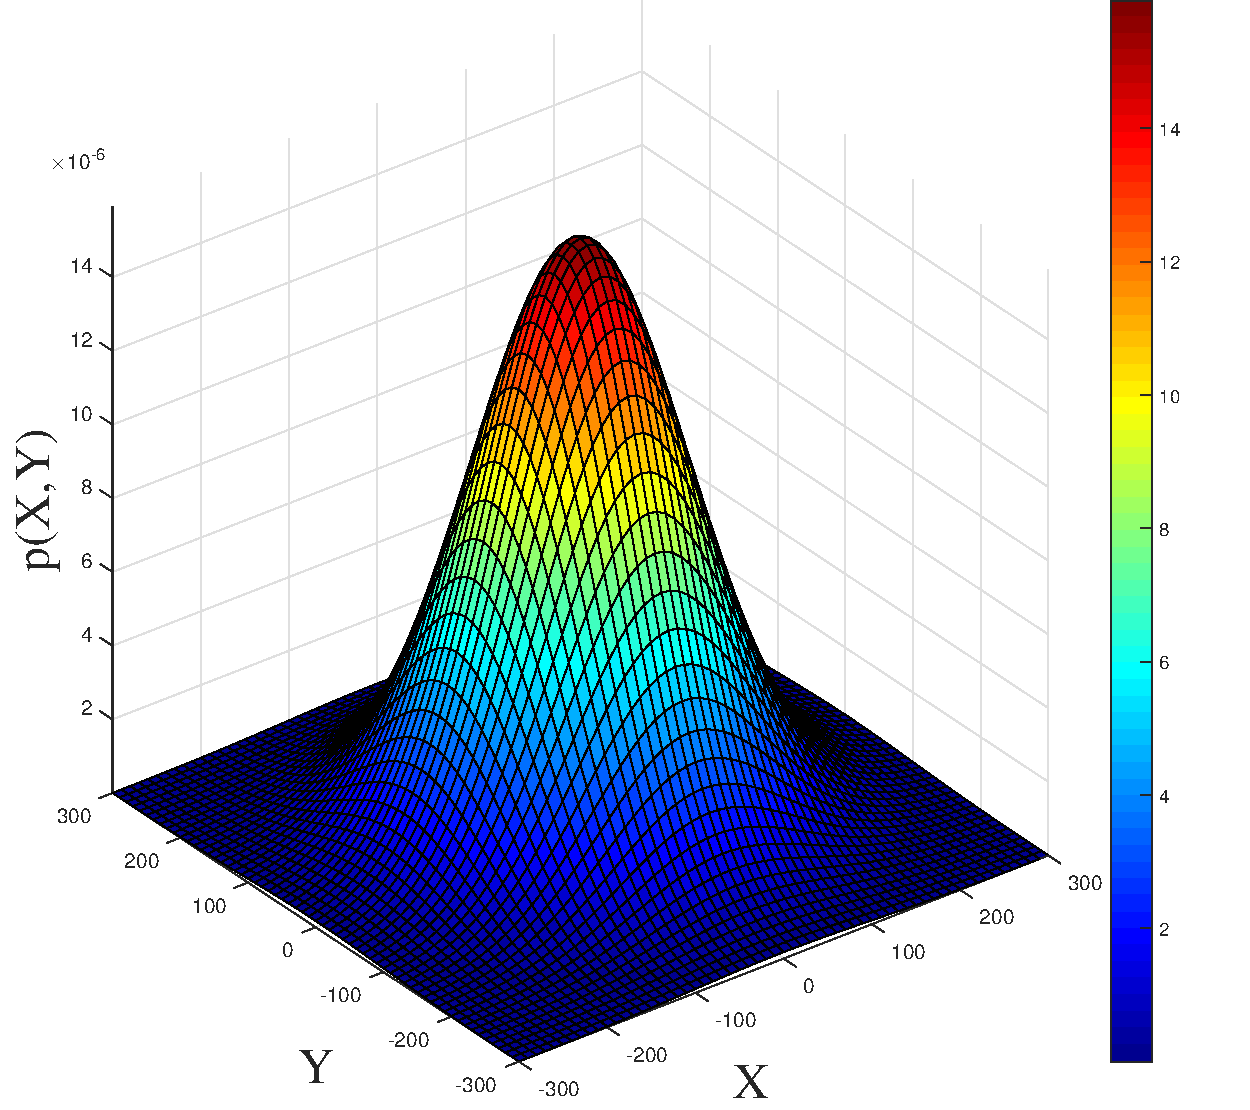
\includegraphics[width=4in]{imgs/1}
\caption{imgs/2.}
\label{imgs/2}
\end{figure}

The university was formed in 1963 as a federation of three existing colleges. The first of these, New Asia College, was established in 1949 by anti-Communist Confucian scholars from Mainland China amid the revolution there. Among the founders were Ch'ien Mu, Tang Junyi, and Tchang Pi-kai. Curriculum focused particularly on Chinese heritage and social concerns. The early years of this school were tumultuous, with the campus relocating several times between rented premises around Kowloon. Academics there were often self-exiled from the mainland and they struggled financially, with students sometimes sleeping on rooftops and teachers foregoing pay to sustain the college. Funds were gradually raised and the school moved to a new campus in Kau Pui Lung, built with the support of the Ford Foundation, in 1956.

\subsection{Origins--2}
The university was formed in 1963 as a federation of three existing colleges. The first of these, New Asia College, was established in 1949 by anti-Communist Confucian scholars from Mainland China amid the revolution there. Among the founders were Ch'ien Mu, Tang Junyi, and Tchang Pi-kai. Curriculum focused particularly on Chinese heritage and social concerns. The early years of this school were tumultuous, with the campus relocating several times between rented premises around Kowloon. Academics there were often self-exiled from the mainland and they struggled financially, with students sometimes sleeping on rooftops and teachers foregoing pay to sustain the college. Funds were gradually raised and the school moved to a new campus in Kau Pui Lung, built with the support of the Ford Foundation, in 1956.

The university was formed in 1963 as a federation of three existing colleges. The first of these, New Asia College, was established in 1949 by anti-Communist Confucian scholars from Mainland China amid the revolution there. Among the founders were Ch'ien Mu, Tang Junyi, and Tchang Pi-kai. Curriculum focused particularly on Chinese heritage and social concerns. The early years of this school were tumultuous, with the campus relocating several times between rented premises around Kowloon. Academics there were often self-exiled from the mainland and they struggled financially, with students sometimes sleeping on rooftops and teachers foregoing pay to sustain the college. Funds were gradually raised and the school moved to a new campus in Kau Pui Lung, built with the support of the Ford Foundation, in 1956.

\begin{figure}[t]
\centering
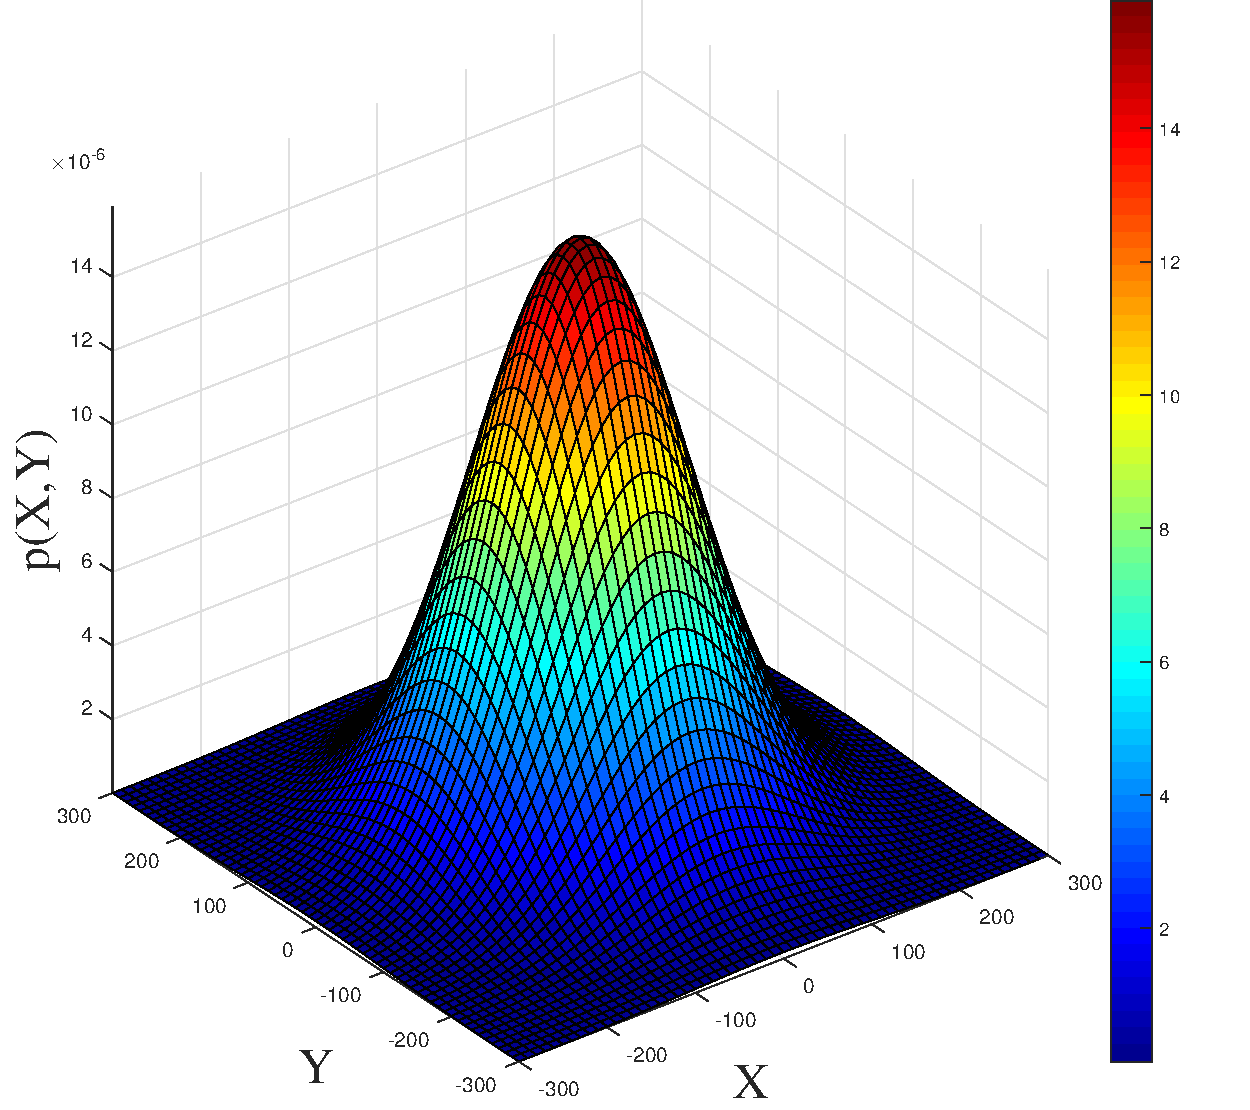
\includegraphics[width=5.5in]{imgs/1}
\caption{imgs/3.}
\label{imgs/3}
\end{figure}

The university was formed in 1963 as a federation of three existing colleges. The first of these, New Asia College, was established in 1949 by anti-Communist Confucian scholars from Mainland China amid the revolution there. Among the founders were Ch'ien Mu, Tang Junyi, and Tchang Pi-kai. Curriculum focused particularly on Chinese heritage and social concerns. The early years of this school were tumultuous, with the campus relocating several times between rented premises around Kowloon. Academics there were often self-exiled from the mainland and they struggled financially, with students sometimes sleeping on rooftops and teachers foregoing pay to sustain the college. Funds were gradually raised and the school moved to a new campus in Kau Pui Lung, built with the support of the Ford Foundation, in 1956.

The university was formed in 1963 as a federation of three existing colleges. The first of these, New Asia College, was established in 1949 by anti-Communist Confucian scholars from Mainland China amid the revolution there. Among the founders were Ch'ien Mu, Tang Junyi, and Tchang Pi-kai. Curriculum focused particularly on Chinese heritage and social concerns. The early years of this school were tumultuous, with the campus relocating several times between rented premises around Kowloon. Academics there were often self-exiled from the mainland and they struggled financially, with students sometimes sleeping on rooftops and teachers foregoing pay to sustain the college. Funds were gradually raised and the school moved to a new campus in Kau Pui Lung, built with the support of the Ford Foundation, in 1956.

The university was formed in 1963 as a federation of three existing colleges. The first of these, New Asia College, was established in 1949 by anti-Communist Confucian scholars from Mainland China amid the revolution there. Among the founders were Ch'ien Mu, Tang Junyi, and Tchang Pi-kai. Curriculum focused particularly on Chinese heritage and social concerns. The early years of this school were tumultuous, with the campus relocating several times between rented premises around Kowloon. Academics there were often self-exiled from the mainland and they struggled financially, with students sometimes sleeping on rooftops and teachers foregoing pay to sustain the college. Funds were gradually raised and the school moved to a new campus in Kau Pui Lung, built with the support of the Ford Foundation\cite{sadri2011logic}, in 1956\cite{sadri2011logic}.
\cite{sadri2011logic}proposed in \cite{heinze2004modelling}

\section{Foundation}
\subsection{Foundation--1}
The university was formed in 1963 as a federation of three existing colleges. The first of these, New Asia College, was established in 1949 by anti-Communist Confucian scholars from Mainland China amid the revolution there. Among the founders were Ch'ien Mu, Tang Junyi, and Tchang Pi-kai. Curriculum focused particularly on Chinese heritage and social concerns. The early years of this school were tumultuous, with the campus relocating several times between rented premises around Kowloon. Academics there were often self-exiled from the mainland and they struggled financially, with students sometimes sleeping on rooftops and teachers foregoing pay to sustain the college. Funds were gradually raised and the school moved to a new campus in Kau Pui Lung, built with the support of the Ford Foundation, in 1956.
\begin{table}[t]
	\caption{Table:1}
	\label{Table:1}       % Give a unique label
	\centering
	\begin{tabular}{ccccc}
		\hline\noalign{\smallskip}
		AS1 & AS2 &AS3  \\
		\noalign{\smallskip}\hline\noalign{\smallskip}
		1 & High 2	& 3\\
		\noalign{\smallskip}\hline
	\end{tabular}
\end{table}
\subsection{Foundation--2}
The university was formed in 1963 as a federation of three existing colleges. The first of these, New Asia College, was established in 1949 by anti-Communist Confucian scholars from Mainland China amid the revolution there. Among the founders were Ch'ien Mu, Tang Junyi, and Tchang Pi-kai. Curriculum focused particularly on Chinese heritage and social concerns. The early years of this school were tumultuous, with the campus relocating several times between rented premises around Kowloon. Academics there were often self-exiled from the mainland and they struggled financially, with students sometimes sleeping on rooftops and teachers foregoing pay to sustain the college. Funds were gradually raised and the school moved to a new campus in Kau Pui Lung, built with the support of the Ford Foundation, in 1956.

\begin{table}[t]
	\caption{Table:2}
	\label{Table:2}       % Give a unique label
	\centering
	\begin{tabular}{ccccc}
		\hline\noalign{\smallskip}
		AS1 & AS2 &AS3  \\
		\noalign{\smallskip}\hline\noalign{\smallskip}
		1 & High 2	& 3\\
		\noalign{\smallskip}\hline
	\end{tabular}
\end{table}

